%!TEX root =  ../thesis.tex
% CHAPTER 2
\chapter{Literature Review}
\label{chp:b2}

	In this chapter, I will explore the existing approaches used by designers to make sense of unfamiliar contexts \cite{aaltonenHowWeMake2005}.

	\begin{figure}[h!]
	\centering
	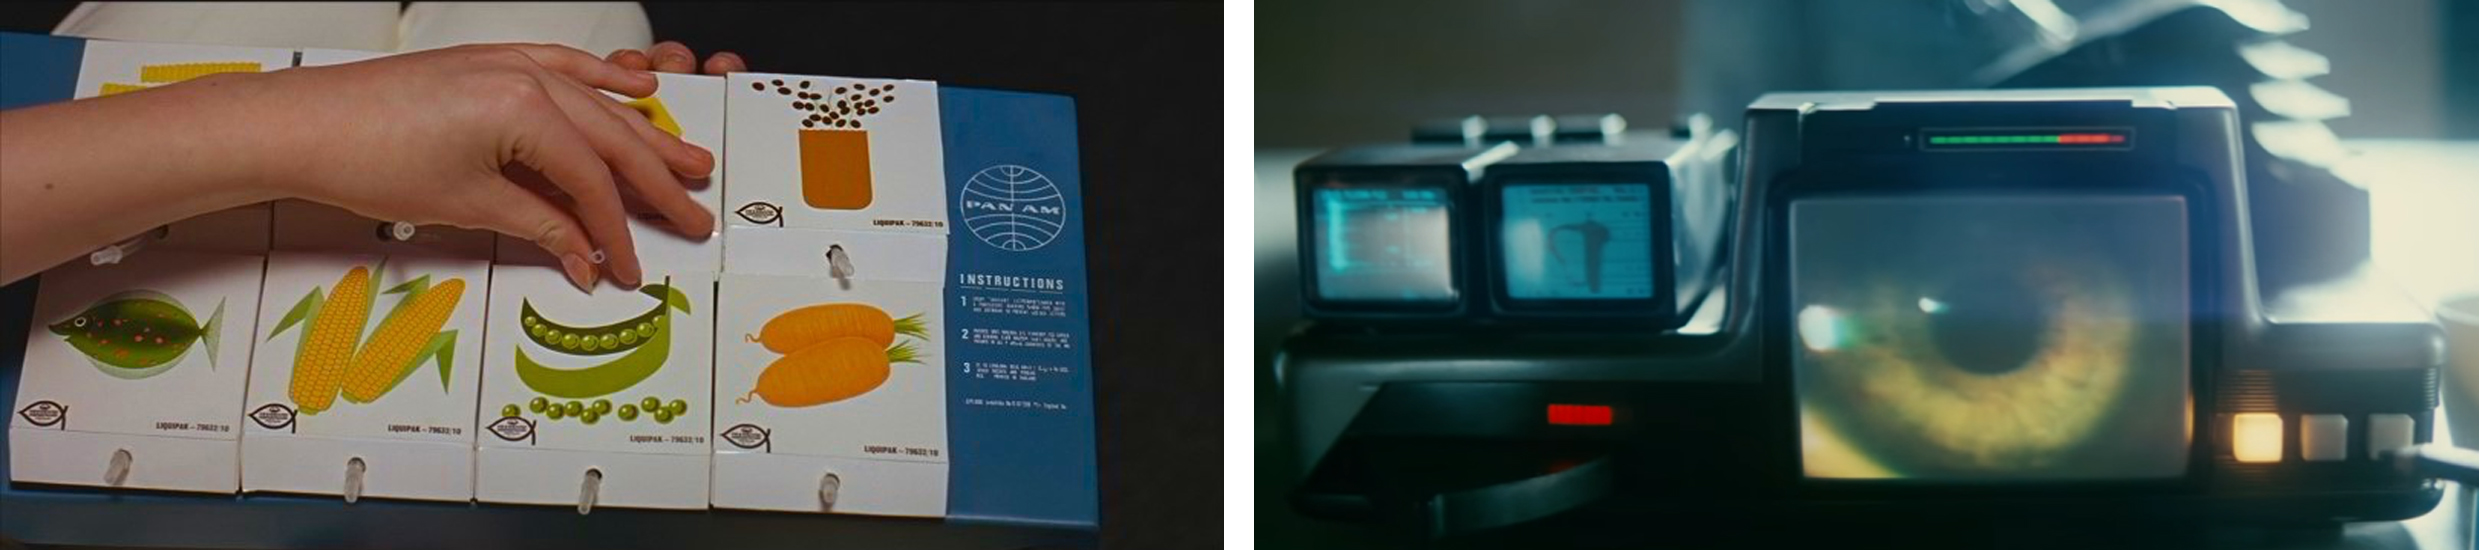
\includegraphics[width=.99\textwidth]{figures/2001-Bladerunner}
	\caption{FFED in the design process.}
	\label{fig:FFED}
	\end{figure}

\section{Heading 1}
Design research is often theorized under three phases: exploratory, generative, and evaluative research.

	\subsection{Subheading}
	\label{subsec:subheading}
	
	\subsubsection{Subsubheading}
	\label{subsubsec:subsubheading}
	Below is a quote I translated from the original Turkish. The original Turkish text is automatically inserted in the Appendix.
	
	\begin{displayquote}
		"English translation from the original quote."\endnote{Orjinal Türkçe metin.}
	\end{displayquote}
	
	Design research is often theorized under three phases: exploratory, generative, and evaluative research \cite{aaltonenHowWeMake2005}. 